% Options for packages loaded elsewhere
\PassOptionsToPackage{unicode}{hyperref}
\PassOptionsToPackage{hyphens}{url}
\PassOptionsToPackage{dvipsnames,svgnames,x11names}{xcolor}
\documentclass[
  10pt,
  a4paper,
]{article}
\usepackage{xcolor}
\usepackage[margin=18mm]{geometry}
\usepackage{amsmath,amssymb}
\setcounter{secnumdepth}{-\maxdimen} % remove section numbering
\usepackage{iftex}
\ifPDFTeX
  \usepackage[T1]{fontenc}
  \usepackage[utf8]{inputenc}
  \usepackage{textcomp} % provide euro and other symbols
\else % if luatex or xetex
  \usepackage{unicode-math} % this also loads fontspec
  \defaultfontfeatures{Scale=MatchLowercase}
  \defaultfontfeatures[\rmfamily]{Ligatures=TeX,Scale=1}
\fi
\usepackage{lmodern}
\ifPDFTeX\else
  % xetex/luatex font selection
  \setmainfont[]{DejaVu Serif}
  \setsansfont[]{DejaVu Sans}
  \setmonofont[]{DejaVu Sans Mono}
\fi
% Use upquote if available, for straight quotes in verbatim environments
\IfFileExists{upquote.sty}{\usepackage{upquote}}{}
\IfFileExists{microtype.sty}{% use microtype if available
  \usepackage[]{microtype}
  \UseMicrotypeSet[protrusion]{basicmath} % disable protrusion for tt fonts
}{}
\makeatletter
\@ifundefined{KOMAClassName}{% if non-KOMA class
  \IfFileExists{parskip.sty}{%
    \usepackage{parskip}
  }{% else
    \setlength{\parindent}{0pt}
    \setlength{\parskip}{6pt plus 2pt minus 1pt}}
}{% if KOMA class
  \KOMAoptions{parskip=half}}
\makeatother
\usepackage{longtable,booktabs,array}
\newcounter{none} % for unnumbered tables
\usepackage{calc} % for calculating minipage widths
% Correct order of tables after \paragraph or \subparagraph
\usepackage{etoolbox}
\makeatletter
\patchcmd\longtable{\par}{\if@noskipsec\mbox{}\fi\par}{}{}
\makeatother
% Allow footnotes in longtable head/foot
\IfFileExists{footnotehyper.sty}{\usepackage{footnotehyper}}{\usepackage{footnote}}
\makesavenoteenv{longtable}
\setlength{\emergencystretch}{3em} % prevent overfull lines
\providecommand{\tightlist}{%
  \setlength{\itemsep}{0pt}\setlength{\parskip}{0pt}}
\usepackage{xeCJK}
\setCJKmainfont[AutoFakeBold=1.4,AutoFakeSlant=0.2]{Droid Sans Fallback}
\setCJKsansfont[AutoFakeBold=1.4,AutoFakeSlant=0.2]{Droid Sans Fallback}
\setCJKmonofont{Droid Sans Fallback}
\emergencystretch=3em
\setlength{\parindent}{0pt}
\xeCJKDeclareCharClass{Default}{"2013,"00B7}
\usepackage{newunicodechar}
\newunicodechar{ℱ}{\ensuremath{\mathcal{F}}}
\renewcommand{\contentsname}{目录}

\usepackage{xurl}

\newunicodechar{ℓ}{\ensuremath{\ell}}
\newunicodechar{𝓕}{\ensuremath{\mathcal{F}}}
\usepackage{pdflscape}
\usepackage{fancyhdr}
\pagestyle{fancy}
\fancyhf{}
\fancyhead[L]{\small PV主线 · 中文审阅草稿}
\fancyhead[R]{\small F仍在执行 · 定量claim未完整复现}
\fancyfoot[C]{\thepage}
\setlength{\headheight}{15pt}
\renewcommand{\headrulewidth}{0.3pt}

\usepackage{graphicx}
\usepackage{bookmark}
\IfFileExists{xurl.sty}{\usepackage{xurl}}{} % add URL line breaks if available
\urlstyle{same}
\hypersetup{
  pdftitle={PV主线中文审阅草稿},
  colorlinks=true,
  linkcolor={Maroon},
  filecolor={Maroon},
  citecolor={Blue},
  urlcolor={Blue},
  pdfcreator={LaTeX via pandoc}}

\title{PV主线中文审阅草稿}
\usepackage{etoolbox}
\makeatletter
\providecommand{\subtitle}[1]{% add subtitle to \maketitle
  \apptocmd{\@title}{\par {\large #1 \par}}{}{}
}
\makeatother
\subtitle{F五组M/L仍在执行；定量核心claim尚未完整复现}
\author{}
\date{2026-09-11 · 保存正文与图件的工作版本}

\begin{document}
\maketitle

{
\setcounter{tocdepth}{1}
\tableofcontents
}
\begin{center}
\fcolorbox{red!70!black}{red!4}{\parbox{0.92\linewidth}{\centering\bfseries 审阅工作稿：F五组M/L仍在执行。\\定量核心claim尚未完整复现，本稿不是最终复现成功报告。}}
\end{center}

当前工作记录，以\href{../PROGRESS.json}{运行索引}和各原式报告为准。目标是闭合原论文Fig.3--11所依赖的有限计算，尤其是同一个完整解上的ρ证据；不是开展新的物理输入或后续算法分支。

\section{1.
已核对的原式与实现}\label{ux5df2ux6838ux5bf9ux7684ux539fux5f0fux4e0eux5b9eux73b0}

原始依据为\href{../../../../references/2309.12402v3.pdf}{2309.12402v3}及其\href{../../../../references/2309.12402v3-source/prd_submission_2.tex}{TeX}，主要为§2.1、§2.3、§3及§4.3。当前PV算子和电流文件身份见\href{../PV_SAME_INPUTS_INVENTORY.md}{清单}。

{\def\LTcaptype{none} % do not increment counter
\begin{longtable}[]{@{}
  >{\raggedright\arraybackslash}p{(\linewidth - 2\tabcolsep) * \real{0.1300}}
  >{\raggedright\arraybackslash}p{(\linewidth - 2\tabcolsep) * \real{0.8700}}@{}}
\toprule\noalign{}
\begin{minipage}[b]{\linewidth}\raggedright
环节
\end{minipage} & \begin{minipage}[b]{\linewidth}\raggedright
原文内容与当前实现
\end{minipage} \\
\midrule\noalign{}
\endhead
\bottomrule\noalign{}
\endlastfoot
完整变量 &
M50给3876个C：T0、100个单密度、2500个ρ1及1275个对称ρ2自由项；加两通道ImF/R各50个后共4076。未降成少数谐波模型。 \\
对称性与分波 &
原文T⁰=3A(s,t,u)+A(t,s,u)+A(u,t,s)，T¹=A(t,s,u)−A(u,t,s)，T²=A(t,s,u)+A(u,t,s)；f=(1/4)∫PℓT。代码\texttt{assemble\_density\_row}与原始角积分有独立检查。 \\
密度坐标 &
数学ρ2上三角的非对角项与C\_flat相差2；\texttt{density\_row\_to\_cflat}及\texttt{coefficient\_blocks}成对处理，L4使用实际密度。不能混同散射双密度ρ与电流谱R。 \\
幺正性 &
κ=π√(1−4/s)，S=1+iκf；原式1−\textbar S\textbar²≥0。L=10为每同位旋10个允许奇偶波，故M50有1500盘。 \\
原生网格 &
\(\phi_j=(j+1/2)\pi/M\)，\(s_j=8/(1+\cos\phi_j)\)。M与L含义均与原文Appendix
A一致。 \\
PV核与FF &
K零基索引为\(\widetilde K_{i+j+1}-\widetilde K_{i-j}\)，利用2M周期正好等于原文一基索引式；偶数K̃为零，奇数为cot(mπ/2M)/M。ReF=1+K
ImF，未错误加入散射未减除核的b\_j常数。 \\
散射求积权重 &
Mandelstam核本身有1/π，故midpoint权为\(s_j^{\prime}/M\)；未减除物理节点核为K+b+iI，\(b_j=s_j^{\prime}/(M s_j)\)。 \\
运动学FF &
k₀²=3β/(256π⁵)，k₁²=(s−4)β/(384π⁵)，𝓕=kF。直接平方原文两个𝓕表达式与代码一致。 \\
电流Gram & 原复Hermitian
Gram经固定酉变换得到实对称矩阵，条目为2−κImf、κImf、κRef、√2kReF、√2kImF及R；代码svec的√2因子逐项匹配。 \\
FESR & 积分不含额外Cauchy
1/π，权为\((\pi/M)s_j^{\prime}s_j^n\)。四矩为S0的n=0,1和P1的n=−1,0；打印归一化矩乘回\(s_0^{n+2}\)。 \\
单位 &
\(s=s_{\mathrm{phys}}/m_\pi^2\)；标量/向量谱分别按mπ⁴/mπ²无量纲化。四个raw矩的物理维数分别为GeV⁶、GeV⁸、GeV²、GeV⁴，不能把同一数值.002写成同一GeV量纲的误差。 \\
FF高能条件 &
仅在原生s\_j\textgreater s0施加\textbar 𝓕₀\textbar²≤2mq²εFF、\textbar 𝓕₁\textbar²≤εFF/2，εFF=6×10⁻⁵；本主线不额外加T0=0或FF无穷远双零。 \\
\end{longtable}
}

F₁(0)=1来自电荷归一化；F₀(0)≈mπ²=1是原文所用的低能近似。这里没有把近似标量关系宣称为精确QCD恒等式。

\section{2.
原文未完全指定的内容必须留在合同中}\label{ux539fux6587ux672aux5b8cux5168ux6307ux5b9aux7684ux5185ux5bb9ux5fc5ux987bux7559ux5728ux5408ux540cux4e2d}

原文明示节点、FF的PV核、原连续色散表示及有限约束，但未给出作者完整的散射交叉核离散代码。仓库的mixed
PV是``原生PV跳跃＋交叉/阈下midpoint有理求积''的具名实现，不能简称为已找回的作者原程序。其有限矩阵证书不证明两种求值规则属于同一个精确解析函数。

本轮按已声明口径固定两个separate-L2手征球、四个raw绝对.002矩误差、hard-midpoint截止和B(M)=100{[}M²+M(M+1)/2{]}的密度L4配方。原文写``some
norm''，未唯一指定该范数；B也不是2309明示参数。历史范数识别参考过输出的事实保留。这些定义使计算可重放，不使来源缺口消失。

GMOR与打印凝聚中心值、共同平均质量下Eq.(2.50)与打印标量矩的差别已\href{../MAINLINE_SOURCE_REVIEW.md}{单列核对}。当前仅使用已经冻结的打印矩，未把两套不相容的误差盒同时施加，也没有为ρ调整质量规则或容差。

因此，不能在结果出来前保证``原文全部量化claim一定复现''。能严格执行的是：明确这些选择，闭合其完整计算链，按结果判断通过或差异，并准确区分来源不足与实现缺陷。

\section{3.
为原型闭环修补的数值问题}\label{ux4e3aux539fux578bux95edux73afux4feeux8865ux7684ux6570ux503cux95eeux9898}

PV
tip已有\href{../PV_tip_support_01/report.json}{完整新中心与支持}，区间\([.09902001731987253,\allowbreak .09911230962662303]\)，\newline gap=9.22923×10⁻⁵。旧PV点仅作为数值初值，其旧中心标签、旧缓存坐标和论文标记ref坐标均未继承。

free-T0
IR旧路径会在已可行点交付前统一缩放，破坏保存中心身份。现已对要求中心的IR通路修正为：先在原H核验，已可行则完整C不变；必须恢复时才走同模型凸段，且取消中心资格。非中心通路保留原有更好incumbent选择。

原subtracted
IR坐标在实际M50计算中两次超过1e−6线性残差门槛；失败记录仍保留。手征增量预条件本身没有解决全部病态性，故进一步采用以下可逆有界坐标，而没有放宽残差或物理条件。

\subsection{保留自由T0的有界坐标证明}\label{ux4fddux7559ux81eaux7531t0ux7684ux6709ux754cux5750ux6807ux8bc1ux660e}

令h=κf。原幺正盘直接给

\[0\le\operatorname{Im}h_{00,j},\operatorname{Im}h_{20,j}\le2,
\qquad -1\le\operatorname{Re}h_{00,a}\le1.\]

取预先固定的中间原生节点\(a=\lfloor M/2\rfloor\)，将这2M+1个量用作自由单密度/T0块的数值坐标。原生虚部对σ的系数是三角块：Imf00的(σ1,σ2)系数为(3/2,1)，Imf20为(0,1)，所以可逆；实S0行的T0系数为5/2，再乘κ\_a\textgreater0后仍非零。于是加入该实部坐标后完整换元可逆。其余3775个实际双密度逐项不变，T0通过逆变换恢复，未被固定为零。

对残差协向量r，包含真实可行域的盒与L4球给

\[h(r)=2\sum_{j<2M}\max(r_j,0)+|r_{2M}|+B\|r_\rho\|_{4/3},\]

\[h(r)+h(-r)=2\sum_{j\le2M}|r_j|+2B\|r_\rho\|_{4/3}.\]

这解释了内部支持与gradient-width公式。代码只在明确由该factory生成的坐标下使用实部{[}-1,1{]}界；固定x再作切片换元。方向恢复后执行原模型线搜索，近中心协向量在原完整坐标重算。最终primal和支持仍回到原H用独立核验，不把浮点内部估计当作最后证书。

\href{../verification_PV_bounded_coordinates.json}{独立检查}包含所有矩阵列的变换对应、原生坐标轴、非零T0往返、密度块不变与原H固定截面支持；当前107项检查、三个测试文件。原始失败、源码字节快照及再运行均保留。

\section{4.
ρ链路的验收条件}\label{ux3c1ux94feux8defux7684ux9a8cux6536ux6761ux4ef6}

代表规则与坐标已在新相位求值前\href{../PV_REPRESENTATIVE_RULE.json}{登记}、\href{../PV_FIXED_COORDINATES.json}{固定}：tip取+x支持；ref取物理Weinberg参考x；mid取此参考与新tip的中点。原文没有给出另外两个代表的精确算法，本规则不冒称作者相同坐标。

依次验收：

\begin{enumerate}
\def\labelenumi{\arabic{enumi}.}
\tightlist
\item
  同一PV
  H下重新求解IR参考点，去除电流条件；初值来自UV不等于IR解仍受UV约束。
\item
  同一H、χ与B下加入100个Gram、四矩和14个FF条件，求解全部C/F/R，而不是从散射点事后补画ρ。
\item
  tip/ref/mid全部达到原式primal、支持间隙和数值中心要求；冻结完整点后再读取相位。图中每条曲线均绑定同一个C/current/joint及其哈希。
\item
  原文§4.3用P1相移经过π/2识别ρ。此处从S本身提取δ、η，报告原生节点括区与描述性插值值；不将F的相位替换为S的相位。
\item
  同时计算\(\mathcal I=|S-1|^2/4\)、向量\textbar F₁\textbar²、两π谱和总电流谱，检查共振增强及谱饱和程度；总谱的全局最大值不被强制与ρ质量精确重合。
\item
  对相邻三点的强度，以原生值包络验证中间值严格高于两侧，得到严格的离散峰证据。任何匹配这些值的连续强度函数必在该括区内部取到最大值；这条条件命题不替代连续物理振幅存在性或唯一极点证明。
\item
  检查同一组完整点的S0/S2，并完成原文M/L配置要求。相位/峰位置的实际变化独立报告；支持gap不是相位误差界，单点峰不是稳定性证明。
\end{enumerate}

\section{5. 当前剩余验收}\label{ux5f53ux524dux5269ux4f59ux9a8cux6536}

IR和UV三代表均已完成中心、原式支持及冻结，原生ρ图和严格峰证据已交付（见后文已闭合结果）；对应的同PV五组M/L链仍在执行。此前analytic-cardinal的图和五组F不能替换这些待完成的PV结果。混合配点原生证据也不会被移交其他插值或用作全能量、无限自旋证书。

只有以上有限主线证据齐备并满足相应物理比较后，才能报告核心复现成功；否则将把具体Major差异、可修补实现问题和原文未充分指定之处分别列出。

\section{本轮IR数值闭合}\label{ux672cux8f6eirux6570ux503cux95edux5408}

PV\_IR\_ref\_04的167步仍未中心收敛，失败及缓存/原C差分留档。复用同H旧IR点前先由PV\_IR\_seed\_replay\_05原式验回，再以标准内侧μ=.01启动新的固定xref、500y目标；χ权重750及全部物理约束保持。PV\_IR\_ref\_05沿中心路径到μ=3.0517578125e−7，原H支持gap=.00159036456423，完整C不作恢复缩放；PV\_IR\_selected核对保存中心与C逐项一致。原式证书与缓存数值中心的范围分别保留。

峰值验证已纳入同一个gauge-phases
CLI：对P1强度的保存f包络及原式K下相同ImF的向量FF平方，严格比较相邻值区间。宽区间不会仅因中值较高就被标作已证峰。该工具未访问新PV相位，不选择新振幅，也不把有限峰升级为唯一物理极点。

预登记旧文本的``Original mixed
collocation''仅按本仓库所声明的有限实现理解，不是作者全代码恢复证据；其中mass\_rule的``average''是文本简称，所有新生产命令及current绑定采用明确的arithmetic-mean。冻结坐标与数值未更改。

\section{原生峰与IR排除的完整短证明}\label{ux539fux751fux5cf0ux4e0eirux6392ux9664ux7684ux5b8cux6574ux77edux8bc1ux660e}

对保存的P1包络f和原生精确s，强度为
I=π²(1−4/s)\textbar f\textbar²/4。Arb计算包含完整包络，不用相位折线反推强度。若
I\_b−I\_a\textgreater0 与 I\_b−I\_c\textgreater0
的区间下界均严格为正，则得到已证离散峰；任何匹配这三个数值的连续I，在紧区间{[}a,c{]}取得最大值，而两端不可能最大，故至少一个内部最大值存在。此结论不声称唯一、非退化、第二张面极点或整个S的连续物理完成。

FF的解析存在性可单独说明：令\(\phi_j=(j+1/2)\pi/M\)、v\_j=ImF\_j，取
\(a_n=(2/M)\sum_j v_j\sin(n\phi_j)\)
(1≤n\textless M)，\(a_M=(1/M)\sum_j v_j\sin(M\phi_j)\)。有限多项式
\(F(z)=1+\sum_{n=1}^M a_n z^n\)
在圆盘内解析。离散正弦正交性给\(\operatorname{Im}F(e^{i\phi_j})=v_j\)；余弦/正弦交叉求和正是原式K，故\(\operatorname{Re}F(e^{i\phi_j})=1+\sum_k K_{jk}v_k\)。因此同一ImF和精确K确实存在连续FF完成，严格邻点差可证明该完成有内部\textbar F\textbar²最大值。该存在性不转移为共同散射函数、全高能FF界或极点证明，也不以任何峰位置筛选振幅。

对IR→UV，若已核验UV对偶给全局支持
n·(x,y)≤U，且冻结IR完整振幅的原H坐标包络满足
n·(x\_IR,y\_IR)−U\textgreater0，则反证法立即排除这个坐标及其完整振幅的任何UV电流扩展。实现使用向外舍入的已证U与原H坐标球，不以某个新电流优化失败代替不可行证明。它不排除整个IR可行集或全部无ρ振幅。

上述FF核等式可直接化为有限三角和：

\[
\begin{aligned}
K_{ki}&=\frac{2}{M}\sum_{n=1}^{M-1}\cos(n\phi_k)\sin(n\phi_i)\\
&=\frac{1}{M}\sum_{n=1}^{M-1}\left[\sin\bigl(n(\phi_i+\phi_k)\bigr)+\sin\bigl(n(\phi_i-\phi_k)\bigr)\right].
\end{aligned}
\]

对整数m，\(\sum_{n=1}^{M-1}\sin(nm\pi/M)\)在m偶数时为0，在m奇数时为cot(mπ/2M)；这由有限等比级数或正弦和公式直接得到。因此\(K_{ki}=\widetilde K_{k+i+1}-\widetilde K_{k-i}\)，与原文(3.67)经一基/零基转换完全相同。Nyquist项n=M的\(\cos(M\phi_k)=0\)，恰解释它只参与虚部重建、系数采用1/M而非2/M。这里没有通过目标ρ曲线识别核。

\section{已闭合的PV主线结果（M50/L10）}\label{ux5df2ux95edux5408ux7684pvux4e3bux7ebfux7ed3ux679cm50l10}

PV\_tip\_support\_01、PV\_UV\_ref\_support\_02、PV\_UV\_mid\_support\_02已全部通过中心、完整primal及支持间隙，并在PV\_UV\_selected冻结后才求相位。IR也已独立冻结。四组各132项原生三主波检查全部sampled\_passed。图和严格峰证据见PV\_native\_phases/phases.json；Fig.7独立交付见PV\_C3\_fig7。

{\def\LTcaptype{none} % do not increment counter
\begin{longtable}[]{@{}
  >{\raggedright\arraybackslash}p{(\linewidth - 8\tabcolsep) * \real{0.0900}}
  >{\raggedleft\arraybackslash}p{(\linewidth - 8\tabcolsep) * \real{0.2600}}
  >{\raggedleft\arraybackslash}p{(\linewidth - 8\tabcolsep) * \real{0.1400}}
  >{\raggedleft\arraybackslash}p{(\linewidth - 8\tabcolsep) * \real{0.2600}}
  >{\raggedleft\arraybackslash}p{(\linewidth - 8\tabcolsep) * \real{0.2500}}@{}}
\toprule\noalign{}
\begin{minipage}[b]{\linewidth}\raggedright
代表
\end{minipage} & \begin{minipage}[b]{\linewidth}\raggedleft
原生90°描述性读数 MeV
\end{minipage} & \begin{minipage}[b]{\linewidth}\raggedleft
min ηP1
\end{minipage} & \begin{minipage}[b]{\linewidth}\raggedleft
P1严格离散主峰 MeV
\end{minipage} & \begin{minipage}[b]{\linewidth}\raggedleft
末层P1最大相移变化
\end{minipage} \\
\midrule\noalign{}
\endhead
\bottomrule\noalign{}
\endlastfoot
tip & 803.386 & .775985 & 792.136 & .04649° \\
mid & 701.114 & .434728 & 680.414 & .24332° \\
ref & 696.561 & .243206 & 680.414 & .11198° \\
\end{longtable}
}

IR最高低能节点的P1为8.56389°。UV的ref与mid支持平面对该IR坐标的严格分离裕量分别为.09777174521与.08328539559，故该完整IR振幅确实不能扩展为满足本UV条件的解。

这闭合了``IR不足、UV排除该IR点并产生共振信号''的有限原型链。强度主峰与向量FF主峰一致的原生节点及严格邻点差均保留；读数不是精确极点质量。三点ρ尺度分散约107
MeV且P1强非弹性，S0/S2亦存在明显分散，原论文的定量合理/稳健曲线claim仍未完整复现，不能把``出现峰''写成全成功。末两层中心的变化小于这些主要差异，但不是整个μ→0误差的严格上界。下一项为同PV五组M/L。

主峰处两π谱份额分别约.86958/.62573/.58204，FF与S相位差分别约−3.168°/−17.973°/−18.977°。对应已保存谱预算在PV\_SPECTRAL\_MECHANISM\_SUMMARY.json。Gram接近行列式饱和不等于R=k²\textbar F\textbar²的纯两π饱和；mid/ref的非弹性与额外谱代价仍显著，不能用``矩阵可行''消除这些物理差异。

三个P1的n=0原始矩均接近同一上边界.1477112，而n=−1矩为.00443585/.00590900/.00608999。由正测度dμ=(R/s)ds，mπ²
I₀/I₋₁是该测度的平均物理能量平方。较大的I₋₁在近乎相同I₀下允许较低平均尺度；这个明确谱预算通道与所见低峰相符，但均值不是峰位公式，也没有证明它是所有差异的唯一原因。原误差盒和全部输入保持不变。

\section{固定μ中心的唯一性与初始化的作用}\label{ux56faux5b9aux3bcux4e2dux5fc3ux7684ux552fux4e00ux6027ux4e0eux521dux59cbux5316ux7684ux4f5cux7528}

这项结论属于当前具名有限模型，不引用旧sine秩证明。密度lift消元后的Hessian为正对角项加正半定外积；其对角系数
\(D_i=2/d_i+8a_i/(\delta+2d_i^2)>0\)，实际密度方向另除B²。因此任意Hessian零方向首先必须有全部δρ=0。散射−log(1−\textbar S\textbar²)的二次块随后要求全部保留δRe
f=δIm
f=0。原生S0/S2虚部对两组单密度的三角块系数为(3/2,1;0,1)，故δσ=0；任一原生S0实部的T0系数5/2非零，故δT0=0。于是C块没有剩余零方向。

在联合模型中，固定δC=0后，低能正定Gram的−logdet二阶型为\(\operatorname{tr}(G^{-1}\delta G\,G^{-1}\delta G)\)，只在δG=0时为零；由其FF虚部条目得到所有低能δImF=0，再由对角谱条目得到δR\_low=0。高能FF盘的二次型控制δF\_high，而ImF\_high直接是其虚部分量，故这些方向也为零。于是活跃变量的完整Hessian正定，限制到固定x截面后仍正定。高能自由R没有被误算进这个唯一性声明。

因此在有严格内点、有限有界活跃域的条件下，每个固定μ\textgreater0及固定正障碍权重对应严格凸的中心问题：若中心存在，其C/ImF/有矩约束R唯一；现有密度/原生盘/正FESR权及FF上界提供活跃变量有界性，标准对数障碍在所声明边界发散，严格内点给出中心的存在性。已保存数值中心通过原式验回；初始化仅是到达该中心的数值手段，旧输出辅助点并不因此获得新代表身份。

这不证明μ→0极值振幅唯一，也不证明作者的未公开障碍权重/正则化选择与本方相同。最后两层中心的可观测量变化另外保存，未把小支持gap当作相位误差定理。自由高能R可有多种完成，原型只保存明确核验的一种；它不改变已冻结C/ImF。

\clearpage
\begin{landscape}
\section*{附图1：Fig.7 IR对照}
\addcontentsline{toc}{section}{附图1：Fig.7 IR对照}
\vfill
\begin{center}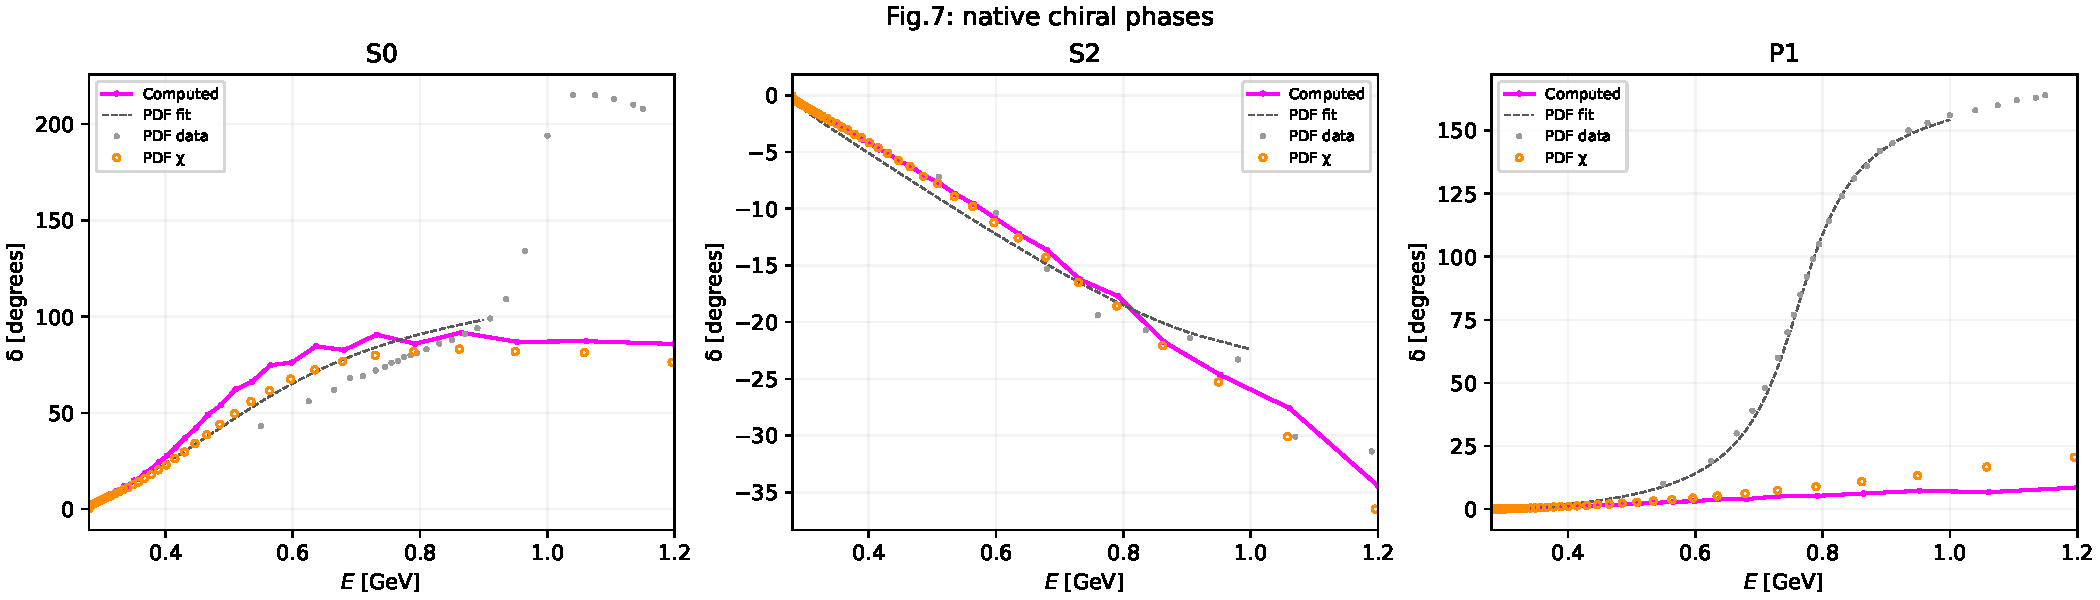
\includegraphics[width=0.98\linewidth]{figures/fig7_IR.pdf}\end{center}
\begin{center}\small 保存图件：\href{../PV_C3_fig7/profiles.pdf}{PV\_C3\_fig7/profiles.pdf}\end{center}
\vfill
\end{landscape}
\clearpage
\section*{附图2：Fig.9 UV相位}
\addcontentsline{toc}{section}{附图2：Fig.9 UV相位}
\vfill
\begin{center}
\includegraphics[width=0.98\linewidth]{figures/fig9.pdf}\end{center}
\begin{center}\small 保存图件：\href{../PV_native_phases/fig9.pdf}{PV\_native\_phases/fig9.pdf}\end{center}
\vfill
\clearpage
\begin{landscape}
\section*{附图3：Fig.10 S0/S2比较}
\addcontentsline{toc}{section}{附图3：Fig.10 S0/S2比较}
\vfill
\begin{center}
\includegraphics[width=0.98\linewidth]{figures/fig10.pdf}\end{center}
\begin{center}\small 保存图件：\href{../PV_native_phases/fig10.pdf}{PV\_native\_phases/fig10.pdf}\end{center}
\vfill
\end{landscape}
\clearpage
\begin{landscape}
\section*{附图4：散射强度、FF与电流谱}
\addcontentsline{toc}{section}{附图4：散射强度、FF与电流谱}
\vfill
\begin{center}
\includegraphics[width=0.98\linewidth]{figures/rho_mechanism.pdf}\end{center}
\begin{center}\small 保存图件：\href{../PV_native_phases/rho_mechanism.pdf}{PV\_native\_phases/rho\_mechanism.pdf}\end{center}
\vfill
\end{landscape}

\end{document}
